\section{Resolución Problema 5}
Dado un numero binario de $n$ bits regresa su equivalente a decimal.


\subsection{\textbf{Descripción del problema:}}

Dar como resultante un numero binario.

\subsection{\textbf{Definición de solución:}}
La solución para convertir un número binario de n bits a su equivalente en decimal consiste en recorrer cada bit del número binario, multiplicar su valor por 2 elevado a la potencia correspondiente según su posición, y sumar los resultados. Al finalizar el recorrido, el valor obtenido será el equivalente decimal del número binario. Es importante verificar la validez del número binario y asegurarse de que esté compuesto únicamente por 0 y 1. El resultado se muestra como el equivalente decimal del número binario.


\subsection{\textbf{Diseño de la solución:}}
El programa solicita al usuario que ingrese un número binario de n bits. Se asegura de que el número ingresado consista únicamente en dígitos binarios 0 y 1. Si se detecta algún dígito decimal, el programa no funcionará.

Luego, se realiza la conversión del número binario ingresado a su equivalente decimal utilizando la fórmula de posición y peso explicada anteriormente.

Finalmente, el programa imprime el resultado de la conversión, es decir, el número decimal equivalente al número binario ingresado por el usuario.


\begin{figure}[H]
    \centering
    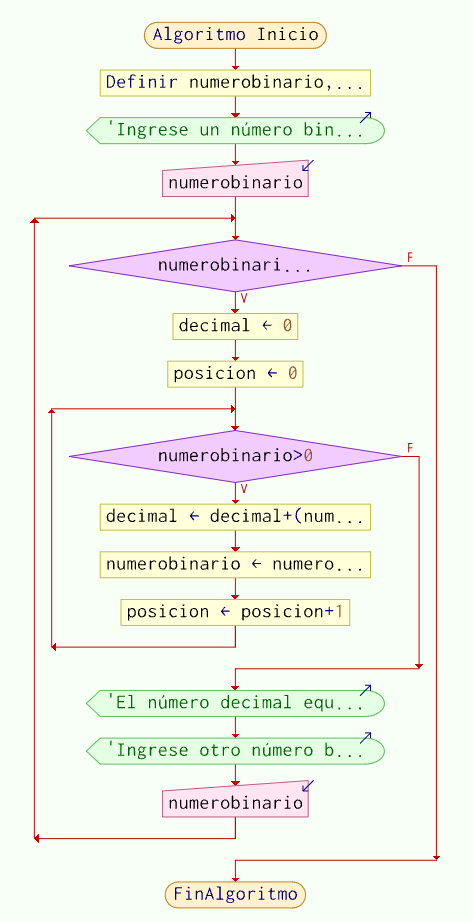
\includegraphics[width=6cm]{Latex-imágenes/ALGORITMO.png}
    \caption{Diagrama de flujo usado como base .}
\end{figure}


\subsection{\textbf{Desarrollo de la solución:}}
El desarrollo del código del programa en Java para la conversión de números binarios a decimales:

\begin{lstlisting}[style=javaStyle]
import java.util.Scanner;
import java.math.BigInteger;

public class NewClass {
    public static void main(String[] args) {
        Scanner bin = new Scanner(System.in);
        boolean continuar = true;
\end{lstlisting}
En esta paso en el programa son colocadas las variables $Scanner$ $BigInteger$
las cuales ayudaran al correr el programa

Se solicita al usuario ingresar un numero binario
\begin{lstlisting}[style=javaStyle]
// Bucle que permite al usuario ingresar números binarios hasta que ingrese 'x'

        while (continuar) {
        
            System.out.print("Ingrese un número en binario (o 'x' para terminar ): ")
            
            String entrada = bin.nextLine();
\end{lstlisting}

 La variable $while$ es utilizada como un "mientras" esta mantiene un bucle regresando a pedirnos un numero binario para su conversión a binario

\begin{lstlisting}[style=javaStyle]
                 // Si se ingresa 'x', el bucle se detiene;
            if (entrada.equalsIgnoreCase("x")) {
                continuar = false;
                continue;
            }
\end{lstlisting}

En esta línea, se declara una variable llamada decimal del tipo BigInteger. Se utiliza para almacenar el valor decimal resultante después de convertir el número binario ingresado. La función convertirBinarioADecimal se llama con el argumento entrada, que es el número binario ingresado por el usuario.

\begin{lstlisting}[style=javaStyle]
 // llama al método convertirBinarioADecimal para convertir el número binario ingresado a decimal
 
            BigInteger decimal = convertirBinarioADecimal(entrada);
            
\end{lstlisting}

 Esta línea imprime en la consola el mensaje "El número en decimal es: " seguido del valor almacenado en la variable decimal. Es decir, muestra el resultado de la conversión en formato decimal.

\begin{lstlisting}[style=javaStyle]
System.out.println("El número en decimal es: " + decimal);

\end{lstlisting}

Estas líneas definen el método convertirBinarioADecimal, que toma un argumento de tipo String llamado binario. El método crea un nuevo objeto BigInteger utilizando el constructor que toma dos argumentos: el número binario (binario) y la base (2) que se utiliza para interpretar el número binario y convertirlo a decimal. 

\begin{lstlisting}[style=javaStyle]
lic static BigInteger convertirBinarioADecimal(String binario) {
        return new BigInteger(binario, 2);

\end{lstlisting}

\text La fórmula se basa en el hecho de que cada posición en un número binario representa una potencia de 2. El dígito en la posición más a la derecha tiene un peso de \(2^0\), el siguiente dígito tiene un peso de \(2^1\), el siguiente tiene un peso de \(2^2\), y así sucesivamente.
\space

\begin{equation}

M = D0 * 2^0 + D1 * 2^1 + D2 * 2^2

\end{equation}


\subsection{\textbf{Depuración y pruebas:}}
En esta tabla se dasarrollan una seria de pruebas, 
\begin{figure}[H]
    \centering
    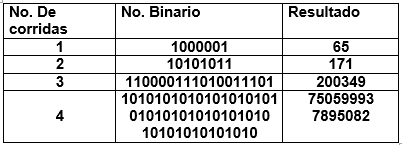
\includegraphics[width=10cm]{Latex-imágenes/TABLA DE PRUEBAS.png}
    \caption{Prueba de escritorio.}
\end{figure}
